\chapter{Ultrafast Carrier Dynamics of (6,5) After Resonant E$_{22}$ Pumping}

\section{Overview}

E22 resonant pump. Spot sizes were . Room temperature, ambient conditions. Dispersion slowly evaporated over time. Normalized data to account for this effect. 

\section{Experimental Results}

\begin{figure}[H]
	\centering
	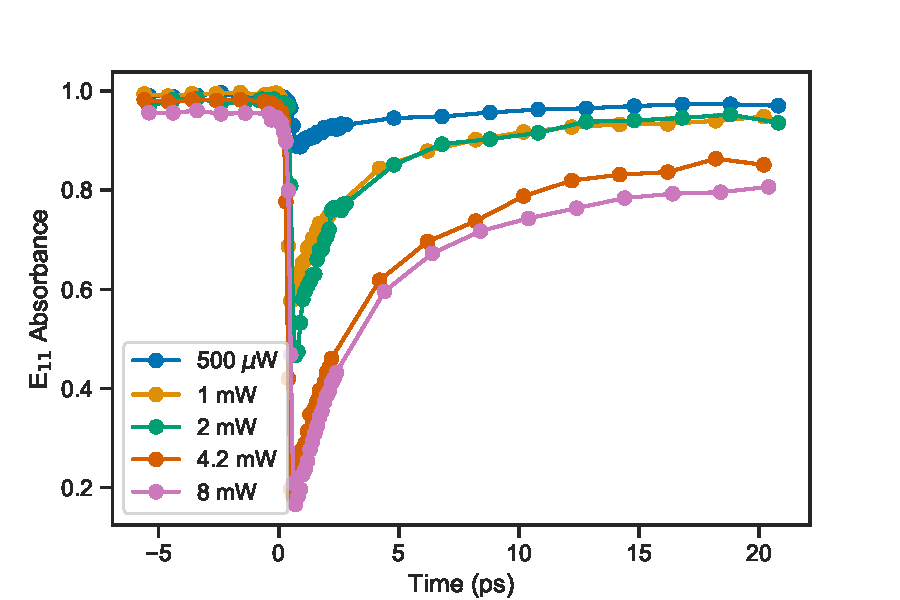
\includegraphics[scale=0.75]{images/chapter_my_data/absorbance_dynamics_E11}
	\caption{Data}
\end{figure}

\begin{figure}[H]
	\centering
	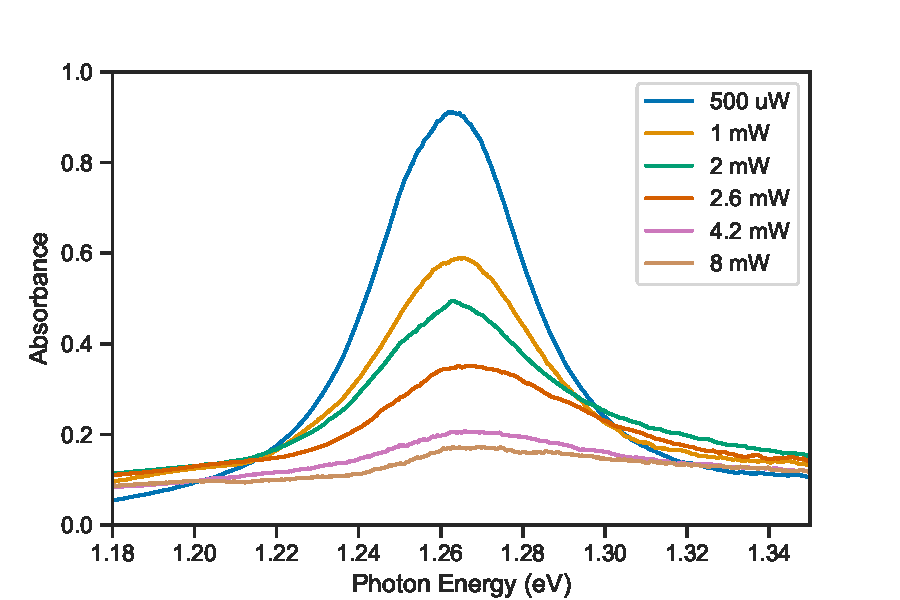
\includegraphics[scale=0.75]{images/chapter_my_data/peak_abs_vs_pump}
	\caption{Data}
\end{figure}

\begin{figure}[H]
	\centering
	\begin{subfigure}{0.46\textwidth}
		\centering
		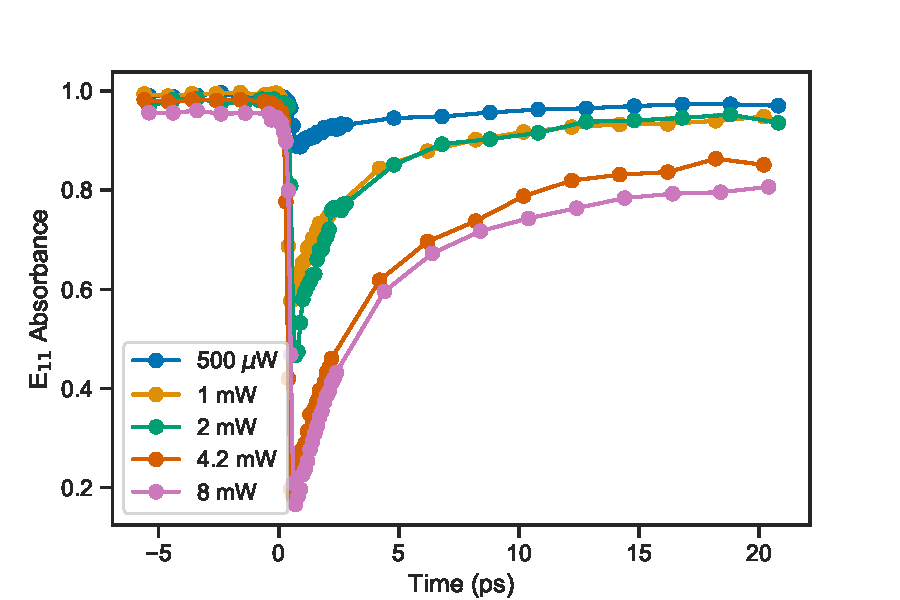
\includegraphics[scale=0.55]{images/chapter_my_data/absorbance_dynamics_E11}
		\caption{A}
	\end{subfigure}
	\qquad
	\centering
	\begin{subfigure}{0.46\textwidth}
		\centering
		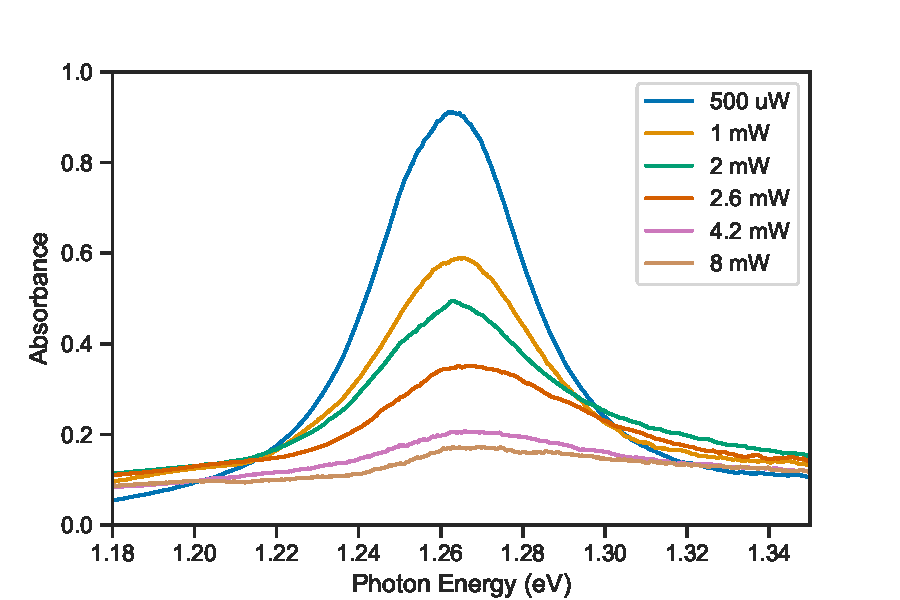
\includegraphics[scale=0.55]{images/chapter_my_data/peak_abs_vs_pump}
		\caption{B}
	\end{subfigure}
	\caption{Data}
\end{figure}

E11 broadens and blueshifts slightly. In data with better signal-to-noise ratio, also observe absorption bleaching of phonon sideband. 

\section{Data Analysis}

Data exhibits bi-exponential decay process.

\begin{figure}[H]
	\centering
	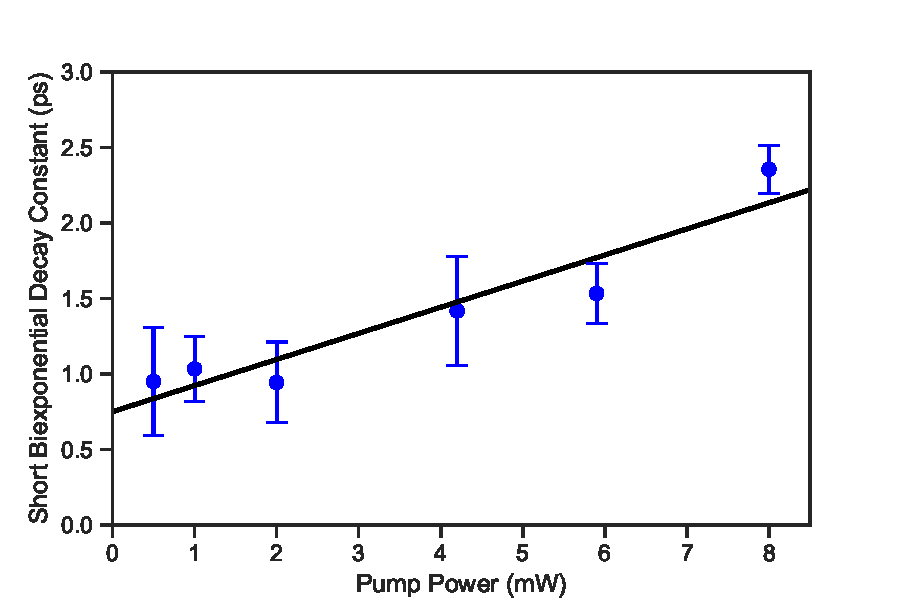
\includegraphics[scale=0.8]{images/chapter_my_data/shorter_biexpconst_fit}
	\caption{Data}
\end{figure}

Only probing bright excitons. 

\section{Discussion}
Exciton-Exciton annihilation supposedly efficient \cite{murakami2009existence}. If this is the case, E11 should not be absorption bleached. 


\section{Conclusions}